\documentclass[11pt,a4paper]{report}
\usepackage[textwidth=37em,vmargin=30mm]{geometry}
\usepackage{calc,xunicode,amsmath,amssymb,paralist,enumitem,tabu,booktabs,datetime2,xeCJK,xeCJKfntef,listings}
\usepackage{tocloft,fancyhdr,tcolorbox,xcolor,graphicx,eso-pic,xltxtra,xelatexemoji}

\newcommand{\envyear}[0]{2025}
\newcommand{\envdatestr}[0]{2025-09-28}
\newcommand{\envfinaldir}[0]{webdb/2025/20250928/final}

\usepackage[hidelinks]{hyperref}
\hypersetup{
    colorlinks=false,
    pdfpagemode=FullScreen,
    pdftitle={Web Digest - \envdatestr}
}

\setlength{\cftbeforechapskip}{10pt}
\renewcommand{\cftchapfont}{\rmfamily\bfseries\large\raggedright}
\setlength{\cftbeforesecskip}{2pt}
\renewcommand{\cftsecfont}{\sffamily\small\raggedright}

\setdefaultleftmargin{2em}{2em}{1em}{1em}{1em}{1em}

\usepackage{xeCJK,xeCJKfntef}
\xeCJKsetup{PunctStyle=plain,RubberPunctSkip=false,CJKglue=\strut\hskip 0pt plus 0.1em minus 0.05em,CJKecglue=\strut\hskip 0.22em plus 0.2em}
\XeTeXlinebreaklocale "zh"
\XeTeXlinebreakskip = 0pt


\setmainfont{Brygada 1918}
\setromanfont{Brygada 1918}
\setsansfont{IBM Plex Sans}
\setmonofont{JetBrains Mono NL}
\setCJKmainfont{Noto Serif CJK SC}
\setCJKromanfont{Noto Serif CJK SC}
\setCJKsansfont{Noto Sans CJK SC}
\setCJKmonofont{Noto Sans CJK SC}

\setlength{\parindent}{0pt}
\setlength{\parskip}{8pt}
\linespread{1.15}

\lstset{
	basicstyle=\ttfamily\footnotesize,
	numbersep=5pt,
	backgroundcolor=\color{black!5},
	showspaces=false,
	showstringspaces=false,
	showtabs=false,
	tabsize=2,
	captionpos=b,
	breaklines=true,
	breakatwhitespace=true,
	breakautoindent=true,
	linewidth=\textwidth
}






\newcommand{\coverpic}[2]{
    % argv: itemurl, authorname
    Cover photo by #2~~(\href{#1}{#1})
}
\newcommand{\makeheader}[0]{
    \begin{titlepage}
        % \newgeometry{hmargin=15mm,tmargin=21mm,bmargin=12mm}
        \begin{center}
            
            \rmfamily\scshape
            \fontspec{BaskervilleF}
            \fontspec{Old Standard}
            \fontsize{59pt}{70pt}\selectfont
            WEB\hfill DIGEST
            
            \vfill
            % \vskip 30pt
            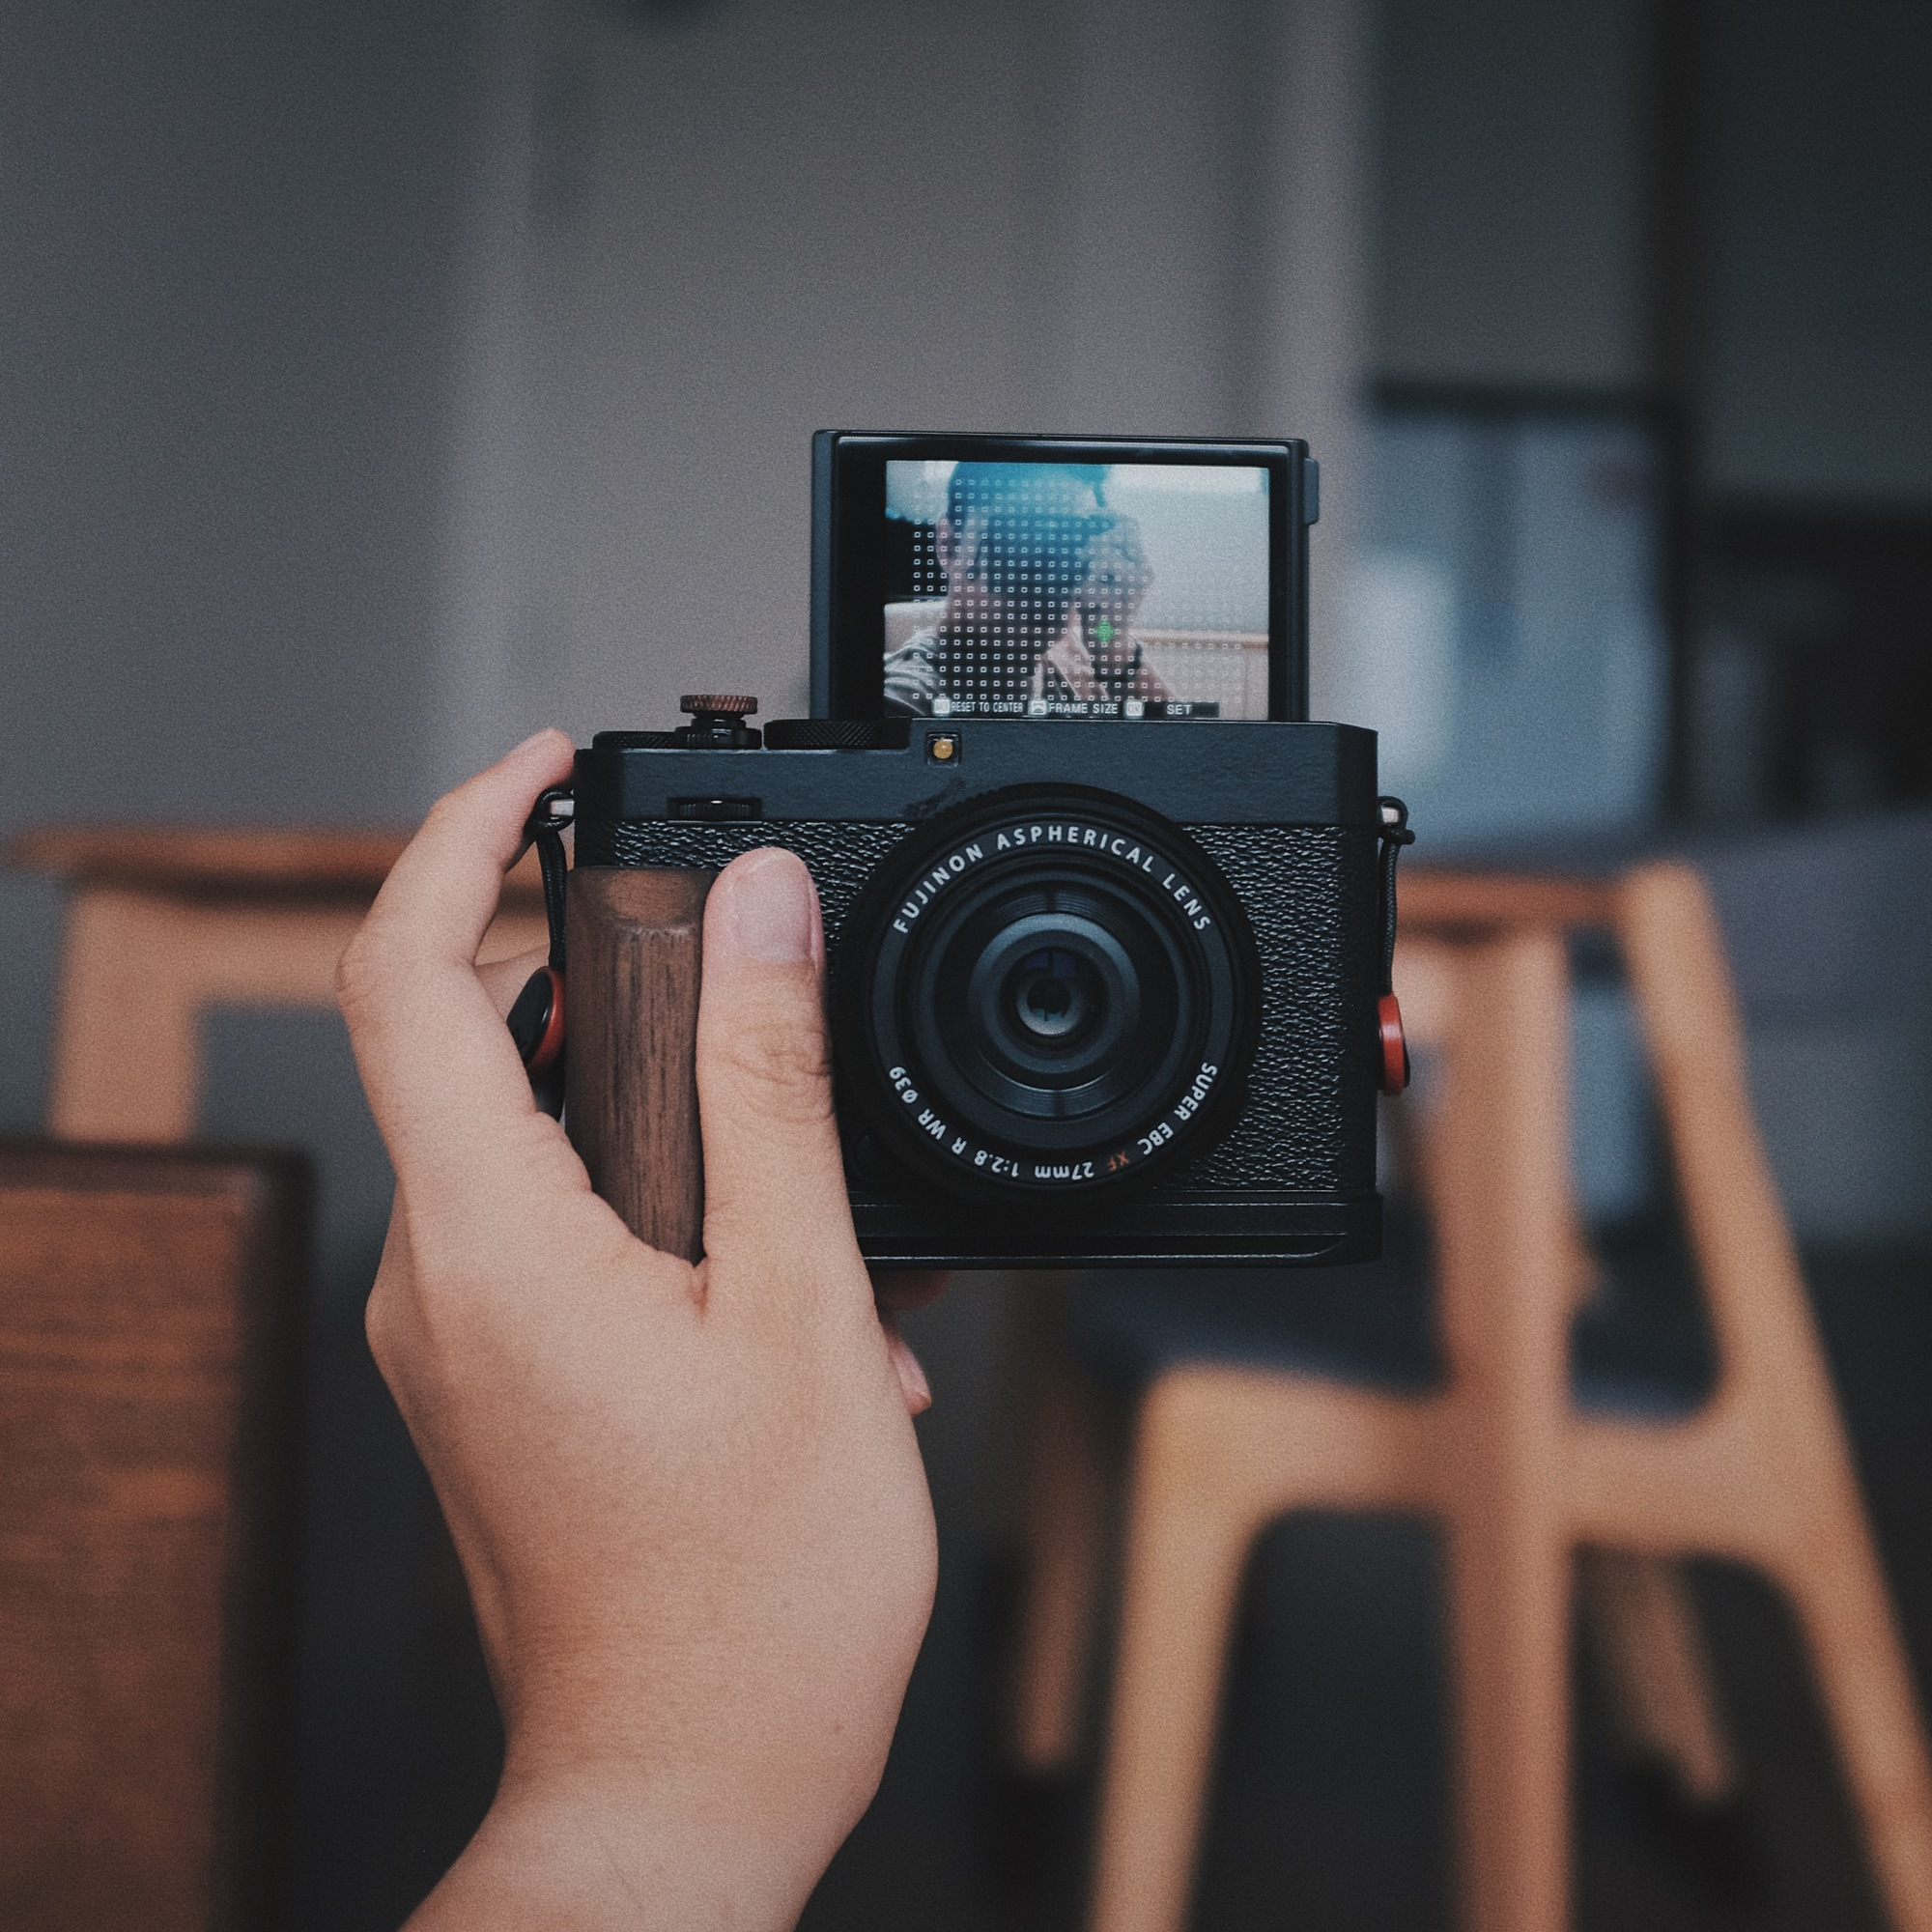
\includegraphics[width=\linewidth]{\envfinaldir/coverpic-prod.jpg}\par
            % \vskip 30pt
            \vfill

            \normalsize\rmfamily\scshape
            \copyright{} The Web Digest Project \hfill\large \envdatestr
        \end{center}
    \end{titlepage}
    % \restoregeometry
}
\newcommand{\simplehref}[1]{%
    \textcolor{blue!80!green}{\href{#1}{#1}}%
}
\renewcommand{\contentsname}{\center\Huge\sffamily\bfseries Contents\par\vskip 20pt}
\newcounter{ipartcounter}
\setcounter{ipartcounter}{0}
\newcommand{\ipart}[1]{
    % \vskip 20pt
    \clearpage
    \stepcounter{ipartcounter}
    \phantomsection
    \addcontentsline{toc}{chapter}{#1}
    % \begin{center}
    %     \Huge
    %     \sffamily\bfseries
    %     #1
    % \end{center}
    % \vskip 20pt plus 7pt
}
\newcounter{ichaptercounter}
\setcounter{ichaptercounter}{0}
\newcommand{\ichapter}[1]{
    % \vskip 20pt
    \clearpage
    \stepcounter{ichaptercounter}
    \phantomsection
    \addcontentsline{toc}{section}{\numberline{\arabic{ichaptercounter}}#1}
    \begin{center}
        \Huge
        \sffamily\bfseries
        #1
    \end{center}
    \vskip 20pt plus 7pt
}
\newcommand{\entrytitlefont}[1]{\subsection*{\raggedright\Large\sffamily\bfseries#1}}
\newcommand{\entryitemGeneric}[2]{
    % argv: title, url
    \parbox{\linewidth}{
        \entrytitlefont{#1}\par\vskip 5pt
        \footnotesize\ttfamily\mdseries
        \simplehref{#2}
    }\vskip 11pt plus 11pt minus 1pt
}
\newcommand{\entryitemGithub}[3]{
    % argv: title, url, desc
    \parbox{\linewidth}{
        \entrytitlefont{#1}\par\vskip 5pt
        \footnotesize\ttfamily\mdseries
        \simplehref{#2}\par\vskip 5pt
        \small\rmfamily\mdseries#3
    }\vskip 11pt plus 11pt minus 1pt
}
\newcommand{\entryitemAp}[3]{
    % argv: title, url, desc
    \parbox{\linewidth}{
        \entrytitlefont{#1}\par\vskip 5pt
        \footnotesize\ttfamily\mdseries
        \simplehref{#2}\par\vskip 5pt
        \small\rmfamily\mdseries#3
    }\vskip 11pt plus 11pt minus 1pt
}
\newcommand{\entryitemHackernews}[3]{
    % argv: title, hnurl, rawurl
    % \parbox{\linewidth}{
    %     \entrytitlefont{#1}\par\vskip 5pt
    %     \footnotesize\ttfamily\mdseries
    %     \simplehref{#3}\par
    %     \textcolor{black!50}{\href{#2}{#2}}
    % }\vskip 11pt plus 11pt minus 1pt
    \begin{minipage}{\linewidth}
            \entrytitlefont{#1}\par\vskip 5pt
            \footnotesize\ttfamily\mdseries
            \simplehref{#3}\par
            \textcolor{black!50}{\href{#2}{#2}}
    \end{minipage}\par\vskip 11pt plus 11pt minus 1pt
}







\begin{document}

\makeheader

\tableofcontents\clearpage




\ipart{Developers}
\ichapter{Hacker News}
\entryitemTwoLinks{iPhone 17 chip becomes the fastest single-core CPU in the world on PassMark}{https://news.ycombinator.com/item?id=45398802}{https://www.tomshardware.com/pc-components/cpus/apples-a19-becomes-the-fastest-single-core-cpu-in-the-world-on-passmark-beating-pc-chips-and-apples-own-m3-ultra-passively-cooled-iphone-17-chip-catapults-past-power-hungry-competitors}

\entryitemTwoLinks{The death of east London's most radical bookshop}{https://news.ycombinator.com/item?id=45398153}{https://www.the-londoner.co.uk/scarlett-letters-closure-left-wing-bookshop/}

\entryitemTwoLinks{I made a public living room and the internet keeps putting weirder stuff in it}{https://news.ycombinator.com/item?id=45398005}{https://www.theroom.lol}

\entryitemTwoLinks{Greenland is a beautiful nightmare}{https://news.ycombinator.com/item?id=45396754}{https://matduggan.com/greenland-is-a-beautiful-nightmare/}

\entryitemTwoLinks{AI model trapped in a Raspberry Pi}{https://news.ycombinator.com/item?id=45396624}{https://blog.adafruit.com/2025/09/26/ai-model-trapped-in-raspberry-pi-piday-raspberrypi/}

\entryitemTwoLinks{A WebGL game where you deliver messages on a tiny planet}{https://news.ycombinator.com/item?id=45396441}{https://messenger.abeto.co/}

\entryitemTwoLinks{Scientists say X has lost its professional edge and Bluesky is taking its place}{https://news.ycombinator.com/item?id=45396377}{https://www.psypost.org/scientists-say-x-formerly-twitter-has-lost-its-professional-edge-and-bluesky-is-taking-its-place/}

\entryitemTwoLinks{Role of Amazon fires in the record atmospheric CO₂ growth in 2024}{https://news.ycombinator.com/item?id=45396284}{https://essopenarchive.org/doi/full/10.22541/essoar.175874118.83695562/v1}

\entryitemTwoLinks{SSH3: Faster and rich secure shell using HTTP/3}{https://news.ycombinator.com/item?id=45395991}{https://github.com/francoismichel/ssh3}

\entryitemTwoLinks{The Postmark backdoor that's downloading emails}{https://news.ycombinator.com/item?id=45395957}{https://www.koi.security/blog/postmark-mcp-npm-malicious-backdoor-email-theft}

\entryitemTwoLinks{Samsung now owns Denon, Bowers and Wilkins, Marantz, Polk, and more audio brands}{https://news.ycombinator.com/item?id=45395396}{https://www.theverge.com/news/784390/samsung-harman-masimo-audio-acquisition-complete}

\entryitemTwoLinks{Ishkur's Guide to Electronic Music}{https://news.ycombinator.com/item?id=45394642}{http://music.ishkur.com/}

\entryitemTwoLinks{Typst: A Possible LaTeX Replacement}{https://news.ycombinator.com/item?id=45393842}{https://lwn.net/Articles/1037577/}

\entryitemTwoLinks{A lifetime of social ties adds up to healthy aging}{https://news.ycombinator.com/item?id=45393501}{https://news.cornell.edu/stories/2025/09/lifetime-social-ties-adds-healthy-aging}

\entryitemTwoLinks{GPT-OSS Reinforcement Learning}{https://news.ycombinator.com/item?id=45392744}{https://docs.unsloth.ai/new/gpt-oss-reinforcement-learning}

\entryitemTwoLinks{The Obsessively Complete Infocom Catalog}{https://news.ycombinator.com/item?id=45392164}{https://eblong.com/infocom/}

\entryitemTwoLinks{New math revives geometry's oldest problems}{https://news.ycombinator.com/item?id=45391871}{https://www.quantamagazine.org/new-math-revives-geometrys-oldest-problems-20250926/}

\entryitemTwoLinks{Why do we remember some life moments but not others?}{https://news.ycombinator.com/item?id=45391786}{https://www.bu.edu/articles/2025/why-do-we-remember-some-moments-but-not-others/}

\entryitemTwoLinks{Thoughts on Mechanical Keyboards and the ZSA Moonlander}{https://news.ycombinator.com/item?id=45391566}{https://www.masteringemacs.org/article/thoughts-on-mechanical-keyboards-zsa-moonlander}

\entryitemTwoLinks{Moondream 3 Preview: Frontier-level reasoning at a blazing speed}{https://news.ycombinator.com/item?id=45391444}{https://moondream.ai/blog/moondream-3-preview}\ichapter{Phoronix}
\entryitemGeneric{\hskip 0pt{}Unvanquished Game Ported To SDL3, Working Natively On Wayland}{https://www.phoronix.com/news/Unvanquished-SDL3-Wayland}

\entryitemGeneric{\hskip 0pt{}Linux Driver Developer At Valve Preps More Patches For Improving AMD GCN 1.0 GPUs}{https://www.phoronix.com/news/AMDGPU-More-GCN-1.0-SI}

\entryitemGeneric{\hskip 0pt{}Linux 6.18 Will Fix Lockups When Systemd Units Read Lots Of Files}{https://www.phoronix.com/news/Linux-6.18-Writeback-Lockups}

\entryitemGeneric{\hskip 0pt{}Btrfs Brings BS Greater Than PS For Linux 6.18, Better Parallelism For Read-Heavy Workloads}{https://www.phoronix.com/news/Linux-6.18-Btrfs}

\entryitemGeneric{\hskip 0pt{}Linux 6.18 sched\_ext Preps For Cgroup Sub-Scheduler Support}{https://www.phoronix.com/news/Linux-6.18-sched-ext}

\entryitemGeneric{\hskip 0pt{}KDE Plasma 6.5 Receives A Grayscale Mode, Early Feature Work Toward Plasma 6.6}{https://www.phoronix.com/news/KDE-Plasma-6.5-Grayscale}

\entryitemGeneric{\hskip 0pt{}Time Is Running Out On Our Autumn Deal To Help Support Linux Hardware Reviews}{https://www.phoronix.com/news/Autumn-2025-Deal-Ending-Soon}

\entryitemGeneric{\hskip 0pt{}GNOME's libadwaita Introduces Adaptive Sidebar Widget}{https://www.phoronix.com/news/GNOME-AdwSidebar}

\entryitemGeneric{\hskip 0pt{}Ubuntu 25.10's Only Supported RISC-V Platform: QEMU Virtualization}{https://www.phoronix.com/news/Ubuntu-25.10-RISC-V-QEMU}


\ipart{Developers~~~~(zh-Hans)}
\ichapter{Solidot}
\entryitemGeneric{\hskip 0pt{}树莓派推出 Raspberry Pi 500+}{https://www.solidot.org/story?sid=82434}

\entryitemGeneric{\hskip 0pt{}亚马逊 kindle 竭尽所能打击电子书盗版}{https://www.solidot.org/story?sid=82433}

\entryitemGeneric{\hskip 0pt{}yt-dlp 将需要安装 JS 运行时 Deno}{https://www.solidot.org/story?sid=82432}

\entryitemGeneric{\hskip 0pt{}白蚁会主动清理危害其培育鸡枞菌的有害菌}{https://www.solidot.org/story?sid=82431}

\entryitemGeneric{\hskip 0pt{}Fedora 讨论使用 AI 工具的政策}{https://www.solidot.org/story?sid=82430}

\entryitemGeneric{\hskip 0pt{}PostgreSQL 18 释出}{https://www.solidot.org/story?sid=82429}

\entryitemGeneric{\hskip 0pt{}在笔记本电脑上模拟宇宙}{https://www.solidot.org/story?sid=82428}

\entryitemGeneric{\hskip 0pt{}ROG Xbox Ally X 售价 1000 美元}{https://www.solidot.org/story?sid=82427}

\entryitemGeneric{\hskip 0pt{}OpenAI 准备建造的数据中心消耗的电力相当于纽约和圣迭戈 }{https://www.solidot.org/story?sid=82426}

\entryitemGeneric{\hskip 0pt{}微软禁止以色列国防部使用它的某些云服务}{https://www.solidot.org/story?sid=82425}

\entryitemGeneric{\hskip 0pt{}对 117 岁寿星的 DNA 研究揭示了长寿的线索}{https://www.solidot.org/story?sid=82423}

\entryitemGeneric{\hskip 0pt{}中国学者《科学》论文接受率为北美同行 1/4}{https://www.solidot.org/story?sid=82422}

\entryitemGeneric{\hskip 0pt{}定期锻炼有助于重塑控制心脏的神经}{https://www.solidot.org/story?sid=82421}

\entryitemGeneric{\hskip 0pt{}英特尔与苹果洽谈投资和加强合作}{https://www.solidot.org/story?sid=82420}

\entryitemGeneric{\hskip 0pt{}微软将让 Copilot 在用户注视下控制浏览器完成各种任务}{https://www.solidot.org/story?sid=82419}

\entryitemGeneric{\hskip 0pt{}俄罗斯卫星带着 75 只老鼠 1500 只果蝇返回地面}{https://www.solidot.org/story?sid=82418}

\entryitemGeneric{\hskip 0pt{}人类骨骼内部发现微塑料}{https://www.solidot.org/story?sid=82417}

\entryitemGeneric{\hskip 0pt{}中国科学家基于不倒翁结构设计扑翼微飞行器}{https://www.solidot.org/story?sid=82416}

\entryitemGeneric{\hskip 0pt{}安理会讨论 AI 和平利用与风险}{https://www.solidot.org/story?sid=82415}

\entryitemGeneric{\hskip 0pt{}智能手机摄像头能变成高光谱传感器}{https://www.solidot.org/story?sid=82414}\ichapter{V2EX}
\entryitemGeneric{\hskip 0pt{}[生活] 想离婚了,还有不离婚的局部最优解吗}{https://www.v2ex.com/t/1162255}

\entryitemGeneric{\hskip 0pt{}[程序员] 什么情况, 字节火山的免费 token 被盗用了好像}{https://www.v2ex.com/t/1162254}

\entryitemGeneric{\hskip 0pt{}[问与答] 请教 V 友,有没有防风 1cc,重量 250g 以内的通勤裤子?}{https://www.v2ex.com/t/1162252}

\entryitemGeneric{\hskip 0pt{}[Steam] 关于游玩刀塔 2 人机开房问题}{https://www.v2ex.com/t/1162251}

\entryitemGeneric{\hskip 0pt{}[问与答] IOS 上有基于 iCloud 什么支持加密的``网盘''软件 适合储存隐私内容的}{https://www.v2ex.com/t/1162250}

\entryitemGeneric{\hskip 0pt{}[问与答] 网络暴力案件被出具不予处罚决定,想问问怎么办}{https://www.v2ex.com/t/1162249}

\entryitemGeneric{\hskip 0pt{}[Java] Java 25 后的时代:像写 Python 一样写 Java}{https://www.v2ex.com/t/1162247}

\entryitemGeneric{\hskip 0pt{}[旅行] [国庆出游]求旅行背包推荐}{https://www.v2ex.com/t/1162246}

\entryitemGeneric{\hskip 0pt{}[问与答] 咨询一下各位:最近给一个政府类 APP 做无障碍测试,这一类的工作可以算是志愿者行为吗?}{https://www.v2ex.com/t/1162245}

\entryitemGeneric{\hskip 0pt{}[程序员] 有逆向 Perimeterx,Datadome 的技术人才吗?}{https://www.v2ex.com/t/1162244}

\entryitemGeneric{\hskip 0pt{}[Apple] 去 apple 换个电池差点被气死}{https://www.v2ex.com/t/1162243}

\entryitemGeneric{\hskip 0pt{}[问与答] 红米平板 Pro 谷歌验证器不能扫码,点击``Scan QR Code''就报错``出了点问题'',怎么破?}{https://www.v2ex.com/t/1162241}

\entryitemGeneric{\hskip 0pt{}[iPhone] 求推荐一个轻薄防指纹磁吸手机壳}{https://www.v2ex.com/t/1162240}

\entryitemGeneric{\hskip 0pt{}[程序员] mantine UI 库和 shadcn UI 库 选哪个?}{https://www.v2ex.com/t/1162238}

\entryitemGeneric{\hskip 0pt{}[职场话题] 职业生涯有些崩了,找心理咨询有帮助吗?}{https://www.v2ex.com/t/1162237}

\entryitemGeneric{\hskip 0pt{}[职场话题] 深圳一公司国庆前补班一天被员工举报,公司反手调整放假制度,取消 14 天年假福利和所有额外假期}{https://www.v2ex.com/t/1162236}

\entryitemGeneric{\hskip 0pt{}[问与答] 大佬们帮我看下这个主机配置做安卓咋样?}{https://www.v2ex.com/t/1162235}

\entryitemGeneric{\hskip 0pt{}[浏览器] 现在手机上还有什么浏览器,可以像 kiwi 一样安装自己的浏览器插件的?}{https://www.v2ex.com/t/1162234}

\entryitemGeneric{\hskip 0pt{}[问与答] oneplus ace pro 声音或者音频有模块吗}{https://www.v2ex.com/t/1162233}

\entryitemGeneric{\hskip 0pt{}[汽车] 什么时候该买车}{https://www.v2ex.com/t/1162232}

\entryitemGeneric{\hskip 0pt{}[职场话题] 你们都怎么摸鱼的?做自己的项目吗?}{https://www.v2ex.com/t/1162231}

\entryitemGeneric{\hskip 0pt{}[Apple] shadowrocket 小火箭有 macOS 原生版本了}{https://www.v2ex.com/t/1162230}

\entryitemGeneric{\hskip 0pt{}[机械键盘] 求推荐分体键盘 (hhkb 转分体,可接受自定义键}{https://www.v2ex.com/t/1162229}

\entryitemGeneric{\hskip 0pt{}[问与答] 一个关于手机个人流水的问题}{https://www.v2ex.com/t/1162228}

\entryitemGeneric{\hskip 0pt{}[职场话题] 某些国人真的是魔幻}{https://www.v2ex.com/t/1162227}

\entryitemGeneric{\hskip 0pt{}[Apple] 关于 Apple Music 的歌曲过渡}{https://www.v2ex.com/t/1162226}

\entryitemGeneric{\hskip 0pt{}[macOS] 2019 Intel macbook pro 折腾 macOS26,及系统降级备忘}{https://www.v2ex.com/t/1162225}

\entryitemGeneric{\hskip 0pt{}[加密货币] 合约还是不能碰,因为选择了跟单}{https://www.v2ex.com/t/1162224}

\entryitemGeneric{\hskip 0pt{}[宽带症候群] 广东联通看网页抖音评论区图片点开加载慢}{https://www.v2ex.com/t/1162222}

\entryitemGeneric{\hskip 0pt{}[问与答] 求助 | 如何屏蔽垃圾邮件}{https://www.v2ex.com/t/1162221}

\entryitemGeneric{\hskip 0pt{}[分享发现] 🚀 跨平台开源 SSH \& SFTP 客户端 —— Shell360}{https://www.v2ex.com/t/1162219}

\entryitemGeneric{\hskip 0pt{}[问与答] airpodspro2 二手价格是多少}{https://www.v2ex.com/t/1162217}

\entryitemGeneric{\hskip 0pt{}[问与答] 你们的土区 AppStore 都低价订阅了什么?}{https://www.v2ex.com/t/1162216}

\entryitemGeneric{\hskip 0pt{}[上海] 上海-古美地区莲花路东兰路俩室一厅整租。}{https://www.v2ex.com/t/1162214}

\entryitemGeneric{\hskip 0pt{}[Android] 小米 17 去实体店摸了下,感觉还不错啊}{https://www.v2ex.com/t/1162213}

\entryitemGeneric{\hskip 0pt{}[WireGuard] Wirguard IPv6 过墙会被阻断吗}{https://www.v2ex.com/t/1162212}

\entryitemGeneric{\hskip 0pt{}[iOS] 圈 X 上 B 站去广告的脚本好像用不了了,还有什么别的法子吗?}{https://www.v2ex.com/t/1162211}

\entryitemGeneric{\hskip 0pt{}[问与答] 没有国外银行卡,怎么买 gpt5 会员?}{https://www.v2ex.com/t/1162210}

\entryitemGeneric{\hskip 0pt{}[iPhone] iPhone 有没有磁吸带线充电宝,有开关可以选择无线充还是有线充}{https://www.v2ex.com/t/1162209}

\entryitemGeneric{\hskip 0pt{}[问与答] 各地路边摊越来越多,实体店面确实夹缝中生存!}{https://www.v2ex.com/t/1162208}

\entryitemGeneric{\hskip 0pt{}[问与答] 机场订阅链接失效、win 平台节点分组分流规则维护这两个痛点有什么解决方案吗}{https://www.v2ex.com/t/1162205}

\entryitemGeneric{\hskip 0pt{}[问与答] 我刚才提问为何大家看不到我提到问题。这儿新用户注册多久才能写长文章啊?}{https://www.v2ex.com/t/1162204}

\entryitemGeneric{\hskip 0pt{}[投资] 利得税的问题}{https://www.v2ex.com/t/1162203}

\entryitemGeneric{\hskip 0pt{}[问与答] 求推荐 AI 搜索览器插件}{https://www.v2ex.com/t/1162202}

\entryitemGeneric{\hskip 0pt{}[Apple] 关于临时解决 MacOS 26 版本 MacBook Chrome 在全屏下标签页右键菜单不显示问题。}{https://www.v2ex.com/t/1162201}

\entryitemGeneric{\hskip 0pt{}[Solana] [不懂就问] 如何把手上的人民币换成\$V2EX}{https://www.v2ex.com/t/1162198}

\entryitemGeneric{\hskip 0pt{}[NAS] 吐槽:飞牛挂载夸克不稳定}{https://www.v2ex.com/t/1162196}

\entryitemGeneric{\hskip 0pt{}[问与答] 在国外,无法登录云闪付有没有解决方法?}{https://www.v2ex.com/t/1162195}

\entryitemGeneric{\hskip 0pt{}[macOS] 更新 macOS 26 后,鼠标经常消失}{https://www.v2ex.com/t/1162194}

\entryitemGeneric{\hskip 0pt{}[汽车] 为什么男生那么看重先买车?}{https://www.v2ex.com/t/1162193}


\ipart{Generic News}







\clearpage
\leavevmode\vfill
\footnotesize

Copyright \copyright{} 2023-2025 Neruthes and other contributors.

This document is published with CC BY-NC-ND 4.0 license.

The entries listed in this newsletter may be copyrighted by their respective creators.

This newsletter is generated by the Web Digest project.

The newsletters are also delivered via Telegram channel \CJKunderline{\href{https://t.me/webdigestchannel}{https://t.me/webdigestchannel}}.\\
RSS feed is available at \CJKunderline{\href{https://webdigest.pages.dev/rss.xml}{https://webdigest.pages.dev/rss.xml}}.

This newsletter is available in PDF at
\CJKunderline{\href{https://webdigest.pages.dev/}{https://webdigest.pages.dev/}}.

The source code being used to generate this newsletter is available at\\
\CJKunderline{\href{https://github.com/neruthes/webdigest}{https://github.com/neruthes/webdigest}}.

This newsletter is also available in
\CJKunderline{\href{http://webdigest.pages.dev/readhtml/\envyear/WebDigest-20250928.html}{HTML}} and
\CJKunderline{\href{https://github.com/neruthes/webdigest/blob/master/markdown/\envyear/WebDigest-20250928.md}{Markdown}}.


\coverpic{https://unsplash.com/photos/street-sign-for-democracy-burning-at-night-9xojIuTqumg}{Steve Johnson}


\end{document}
